% \appendix

% #📘 appendix-ch4-channel-estimation-equalization.tex

\chapterAppendix: Channel Estimation and Equalization}
%\label{appendix:channel_estimation}

This appendix supplements Chapter 4 by providing a practical demonstration of channel estimation and equalization techniques used in modern OFDM systems like LTE and 5G NR.

\subsection{Notebook Simulation: \texttt{A4\_channel\_equalization.ipynb}}

The notebook implements the following:

\begin{itemize}
  \item QPSK modulation over 64 OFDM subcarriers.
  \item Addition of a cyclic prefix and multipath channel convolution.
  \item Complex AWGN noise addition.
  \item Channel estimation using Least Squares (LS) method.
  \item Equalization and recovery of original QPSK symbols.
\end{itemize}

The simulation assumes pilot-based LS estimation and perfect channel knowledge at the receiver for educational clarity.

\subsection{Streamlit App (Optional)}
For interactive learning, a Streamlit-based simulation page may be included in the modular app to vary parameters like channel taps, SNR, and modulation order.

\subsection{Visualization of Equalized Symbols}

Figure~\ref{fig:equalized-constellation} shows the scatter plot of the received frequency-domain symbols and the equalized output after applying channel estimation.

\begin{figure}[H]
    \centering
    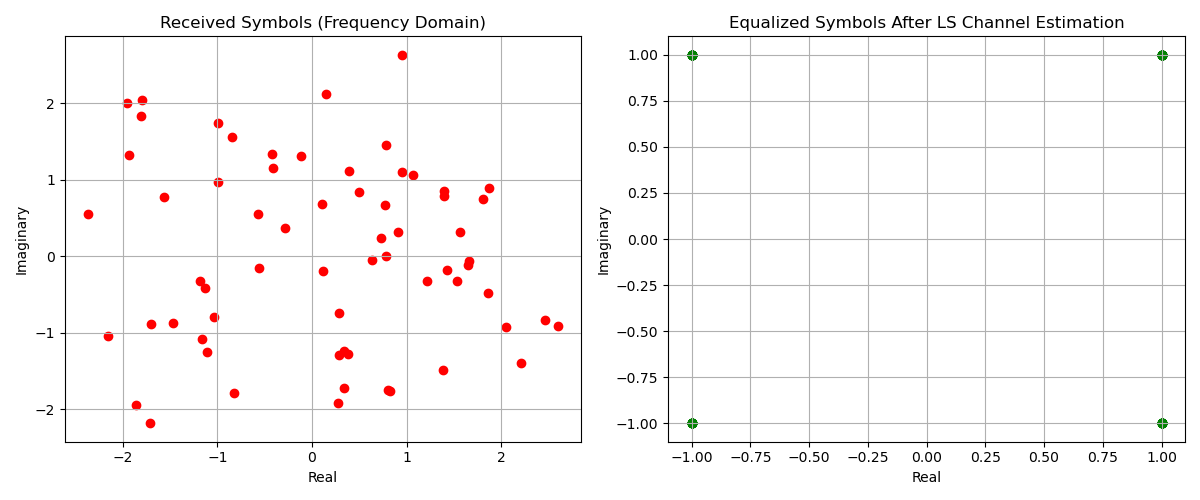
\includegraphics[width=0.75\textwidth]{./figures/equalized_constellation.png}
    \caption{Constellation plot of received vs. equalized QPSK symbols.}
    \label{fig:equalized-constellation}
\end{figure}

\subsection*{References}
\begin{enumerate}
    \item Rappaport, T. S. \textit{Wireless Communications: Principles and Practice}, Pearson.
    \item Goldsmith, A. \textit{Wireless Communications}, Cambridge University Press.
    \item Proakis, J. G., \textit{Digital Communications}.
    \item 3GPP TS 36.211: \textit{Physical Channels and Modulation (LTE)}.
\end{enumerate}



\section{Additional Appendix: Channel Estimation and Equalization Simulation}

\subsection{Overview}

This appendix provides a hands-on simulation of OFDM-based channel estimation and equalization using a simple multipath fading channel. The exercises are aimed at helping learners visualize the distortion introduced by the wireless channel and how equalization can recover the original signal.

\subsection{Interactive Notebook: \texttt{A4\_channel\_equalization.ipynb}}

The Jupyter Notebook implements the following:
\begin{itemize}
  \item Generation of QPSK-modulated OFDM symbols
  \item Simulation of a multipath channel with user-defined tap coefficients
  \item Addition of AWGN noise based on a tunable SNR
  \item Least Squares (LS) channel estimation
  \item Equalization of the received signal
  \item Scatter plots comparing received and equalized symbols
\end{itemize}

\noindent
You can access and run the notebook here:

\begin{quote}
\texttt{[Download or open from: A4\_channel\_equalization.ipynb]}
\end{quote}

\subsection{Streamlit App: EqualizerSimulator.py}

A lightweight web interface allows learners to interactively tune parameters like:
\begin{itemize}
  \item Number of subcarriers ($N$)
  \item Cyclic prefix length
  \item SNR (dB)
  \item Complex channel tap coefficients
\end{itemize}

\noindent
Launch the app locally or via cloud deployment to visualize the following:
\begin{enumerate}
  \item Received symbols (with distortion)
  \item Equalized symbols (recovered)
\end{enumerate}

\noindent
\textbf{To launch locally:}
\begin{verbatim}
 streamlit run EqualizerSimulator.py
\end{verbatim}

\subsection{Example Constellation Plot}

\begin{figure}[H]
  \centering
  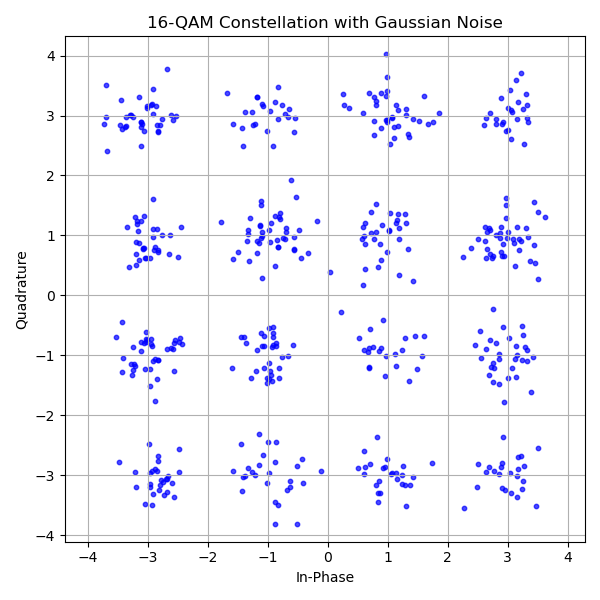
\includegraphics[width=0.7\textwidth]{./figures/modulation_constellation_example.png}
  \caption{Comparison of Received vs Equalized QPSK Symbols}
  \label{fig:equalized_qpsk}
\end{figure}

\subsection{References}
\begin{itemize}
  \item S. Haykin and M. Moher, \textit{Modern Wireless Communications}, Pearson
  \item T. S. Rappaport, \textit{Wireless Communications: Principles and Practice}, Prentice Hall
  \item 3GPP Technical Reports on OFDM and Channel Estimation
  \item MATLAB and Python tutorials on Least Squares Estimation
\end{itemize}


% # ✅ Features:
%  * Adjustable SNR, Cyclic Prefix, and Channel Taps.
%  * Visual comparison: Received symbols vs Equalized symbols.
%  * Uses Least Squares Estimation for channel response.
